\chapter{Experimental Apparatus}
\label{chap:detector}
\begin{comment}
\section{CMS Detector}
The aim of a particle detector is to count the particles produced that pass through it after being produced in a collision or a decay - an ``event'', to visualise their tracks, to measure their energies and momenta, to record time-of-flight and to identify their identity. The exact position where the event occurs is known as the interaction point. It is neccessary to know the mass and momentum of the particles to identify them. The mass can be found by measuring either the velocity or the energy and the momentum. Depending on the type of the particles and forces to be studied, various detectors have been designed.

In particle physics, a hermetic detector, also known as a 4$\pi$ detector, is a particle detector which is designed to observe all possible decay products of an interaction between subatomic particles in a collider. It covers a large area around the interaction point and  consists of layers of sub-detectors each specialising in a particular type of particle or property. They are typically cylindrical having different types of detectors wrapped around each other. These are known as hermetic because their construction is such that the motion of particles is ceased at the boundaries of the chamber and the particles donot move beyond the seals. These detectors cover solid angle nearly of 4$\pi$ steradians around the interaction point and hence are named as ``4$\pi$'' detectors.

The first 4$\pi$ detector was the ``Mark I'' at the Stanford Linear Accelerator Center (SLAC) which resulted in the discoveries of J/$\psi$ particle and $\tau$ lepton. Its basic design has been used for all modern collider detectors. Prior to the building of the Mark I, it was thought that most particle decay products would have relatively low transverse momentum (i.e. momentum perpendicular to the beamline), so that detectors could cover this area only. However, it was learnt at the Mark I and subsequent experiments that the most fundamental particle interactions at colliders involve very large exchanges of energy and therefore involve large transverse momenta. So the large angular coverage is taken into account for modern particle physics.

The modern particle large-scale detectors in use in accelerators such as Large hadron collider at CERN which includes ATLAS and LHCb or HERA at DESY are hermetic detectors. The accelerators and detectors are often situated underground to provide the maximum possible shielding from natural radiations such as cosmic rays. The various particle detectors can be summarised as shown in Figure \ref{summary}.

\begin{figure}[h!]
\begin{center} 
\includegraphics[scale = 0.75]{figs/Detector/detectorsummary.png}
\caption{Summary  of Particle detectors.}
\label{summary}
\end{center}
\end{figure} 

\subsection{Prototype Detector}
The main components of a hermetic or a prototype detector are dicussed below as :
\begin{itemize}
\item
$\bf{Vertex}$ $\bf{detector}$ $\bf{(VDET)}$ - Vertex detector is a high resolution position detector for identifying very short-lived particles. One such detector as shown in Figure \ref{vertex} consists of two concentric arrays of silicon wafers arround the beam pipe. It is designed to identify the location of the collision as closely as possible. The particles leave small electric charges in the squares they cross on traveling through the thin chips. The location of these deposits can be recorded electronically and these can be connected to reconstrust the track of the particles. The electronic squares are very small in size. So the position of the charged particle can be measured with microscopic accuracy, about 200 millionths of an inch. The position where any charged particle has been created i.e. the vertex can be found by drawing each path back to where it meets with one or more paths as the charged particles are always produced in pairs of equal and opposite charges.   
 
\begin{figure}[h!]
\begin{center} 
\includegraphics[scale = 0.75]{figs/Detector/vertex.jpg}
\caption{The Vertex Detector.}
\label{vertex}
\end{center}
\end{figure} 

\item
$\bf{Trackers}$ - A tracking detector reveals the track or path followed by an electrically charged particle by the trails left behind. The tracking system plots the helix path traced by a charged particle that curves in a magnetic field by localizing it in space in finely-segmented layers of detecting material, usually silicon. The modern tracking devices do not make the tracks visible directly. The tiny electric signals are recorded by the computers which are then reconstructed by a computer program and is displayed on the screen. The Inner Track Chamber (ITC) or Central Tracking Detector (CTD) is a large drift chamber crisscrossed with sense wires arranged in concentric cylindrical layers. Whenever a charged particle passes near one of the wires, the electrical properties of a wire change and gets recorded by the computer. The active length of the chamber is few meters and extends in radius between 16 and 26 cm from the beam line. The curvature of the path helps to know the charge and momentum of the particle. A strong magnetic field is used to identify the particles produced as it bends the particle's path into a curve. The degree to which the particle bends is inversely proportional to its transverse momentum. So the particles having very high momentum travel in almost straight lines whereas those with low momentum move forward in tight spirals. The direction in which the particles bend tells about the charge as positive and negative charges curve in opposite directions.


\item
$\bf{Time}$ $\bf{Projection}$ $\bf{Chamber}$  $\bf{(TPC)}$ - Time Projection Chamber (TPC) measures the three dimensional coordinate at many points along the track of a charged particle. When there are large numbers of tracks within a small angular cone, it is important to have the 3-dimensional information. The transverse coordinates are determined by wire proportional chambers at the ends of the TPC while the longitudinal (z) coordinate is obtained from the time taken by the charged particles to drift to the ends of the TPC. This is essentially a larger drift chamber.

\item 
$\bf{Large}$ $\bf{Superconducting}$ $\bf{magnet}$  - This produces a strong magnetic field to curve the tracks of charged particles in the tracking detectors and provides their momenta.

\item 
$\bf{Calorimeters}$ - A calorimeter measures the energy lost by a particle on travelling through it. It is designed to slow down the particles and to absorb their energy into a material. Calorimeters consist of layers of passive or absorbing high-density maerial such as lead having layers of active medium such as solid lead-glass or liquid argon. 
There are two types of calorimeters : 

$\bf{The}$ $\bf{Electromagnetic}$ $\bf{calorimeters}$ $\bf{(ECAL)}$ - The electromagnetic calorimeters measure the energy of light particles - electrons and photons - as they interact electrically with the charged particles inside the matter. Electrons, positrons create a cascade of photons and electron-positron pairs known as electromagnetic shower which spreads due to compton scattering and the photoelecric effect. The photons being neutral donot leave tracks in the CTD but produce an electromagnetic shower in the ECAL. The electrons and positrons, being charged, leave tracks in the CTD and give rise to a shower in the ECAL. 


$\bf{The}$ $\bf{Hadronic}$ $\bf{calorimeters}$ $\bf{(HCAL)}$ - The hadronic calorimeters specialize in absorbing hadrons such as protons and neutrons which interact through the strong nuclear force. The charged hadrons leave track in all the layers of detectors upto the HCAL and deposit all their energy. The neutral hadrons donot leave track in any of the layers of detectors but produce shower and deposit their energy in the HCAL. 

The calorimeters can stop or absorb most of the known particles except muons and neutrinos.

\item
$\bf{Muon}$ $\bf{Chambers}$ - Only the muons and neutrinos, out of all the known stable particles, pass through the calorimeter without depositing most or all of their energy. They interact very little with matter and can travel long distances through the dense matter. The charged muons can be detected my having an additional tracking system outside the calorimeters whereas the neutrinos are practically undetectable as they escape completely without bieng tracked in any of the layers. Their presence can be detected from the missing energy carried by them.

 Many particles donot live long enough to reach the tracking chamber. They can be detected indirectly from the particles they decay into and then knowing the properties of the parent particle by going backwards.

\item
$\bf{Particle}$ $\bf{identification}$ $\bf{detectors}$ - Two methods of particle identification work by detecting radiation emitted by charged particles:

$\bf{Cherenkov}$ $\bf{radiation}$: The cerenkov radiation is the light emitted when a charged particle travels faster than the speed of light through a given medium. The light is given off at a specific angle according to the velocity of the particle. Combined with a measurement of momentum of the particle, velocity can be used to determine the mass and hence to identify the particle.

$\bf{Transition}$ $\bf{radiation}$: The transition radiation is produced by relativistic charged particles as they cross the boundary between two electrical insulators with different resistances to electric currents. The intensity of the emitted radiation is roughly proportional to the energy of the particle. So the transition radiation distinguishes the particles, particularly electrons and hadrons in the momentum range between 1 GeV/c and 100 GeV/c. The probability of transition radiation increases with the relativistic gamma factor $\gamma$ at each interface between materials. Thus particles with large $\gamma$ give off many photons and small 
$\gamma$ give off few. A lighter particle, with high $\gamma$, radiates more as compared to a heavier particle, with low $\gamma$.



\end{itemize}
Figure \ref {detection} shows an example of particles generated after a collision in (a) and the actual display observed in (b).

\begin{figure}[h!]
\begin{center} 
\includegraphics[scale = 0.75]{figs/Detector/detection.jpg}
\caption{An example to show the particles generated after a collision.}
\label{detection}
\end{center}
\end{figure} 

1. Magnetic field bends the low and medium energy charged particles into curved trajectories.\\
2. The filled-in dots represent the charged particles detected by the ionization detectors.\\
3. The smaller size ellipses show the showers (secondary particles) detected by the ECAL.\\
4. The larger size ellipses show the showers detected by the HCAL.\\
5. Three additional dots are from the muon chamber at the outer fringe of the detector.\\
6. The neutrino, which disappears without a trace, can be accounted for from missing energy.\\


The Large Hadron Collider (LHC) ~\cite{LHC} at CERN near Geneva is the world's newest and most powerful tool for Particle Physics research.The LHC is built in a circular tunnel of 27 km in circumference. The tunnel is buried around 50 to 175 m underground. It is designed to collide two counter rotating proton or heavy ion beams with a centre-of-mass energy of 14 TeV and an unprecedented luminosity of 10$^{34}$ cm$^{-2}$ s$^{-1}$. It can also collide heavy (Pb) ions with an energy of 2.8 TeV per nucleon and a peak luminosity of 10$^{27}$ cm$^{-2}$ s$^{-1}$. The two proton beams rotate in opposite directions around the ring as shown in Figure \ref{LHC}, crossing at the designated interaction regions (IRs). The four of these i.e. IR1, IR2, IR5 and IR8 house the various experiments which are ATLAS ~\cite{ATLAS}, LHCf, ALICE ~\cite{ALICE}, CMS ~\cite{CMS}, TOTEM ~\cite{TOTEM} and LHCb ~\cite{LHCb}. IR4 contains the radio-frequency (RF) acceleration equipment and IR3 and IR7 contain equipment for collimation and for protecting the machine from stray beam particles. IR6 houses the beam abort system where the LHC beam can be extracted from the machine. 

\begin{figure}[h!]
\begin{center} 
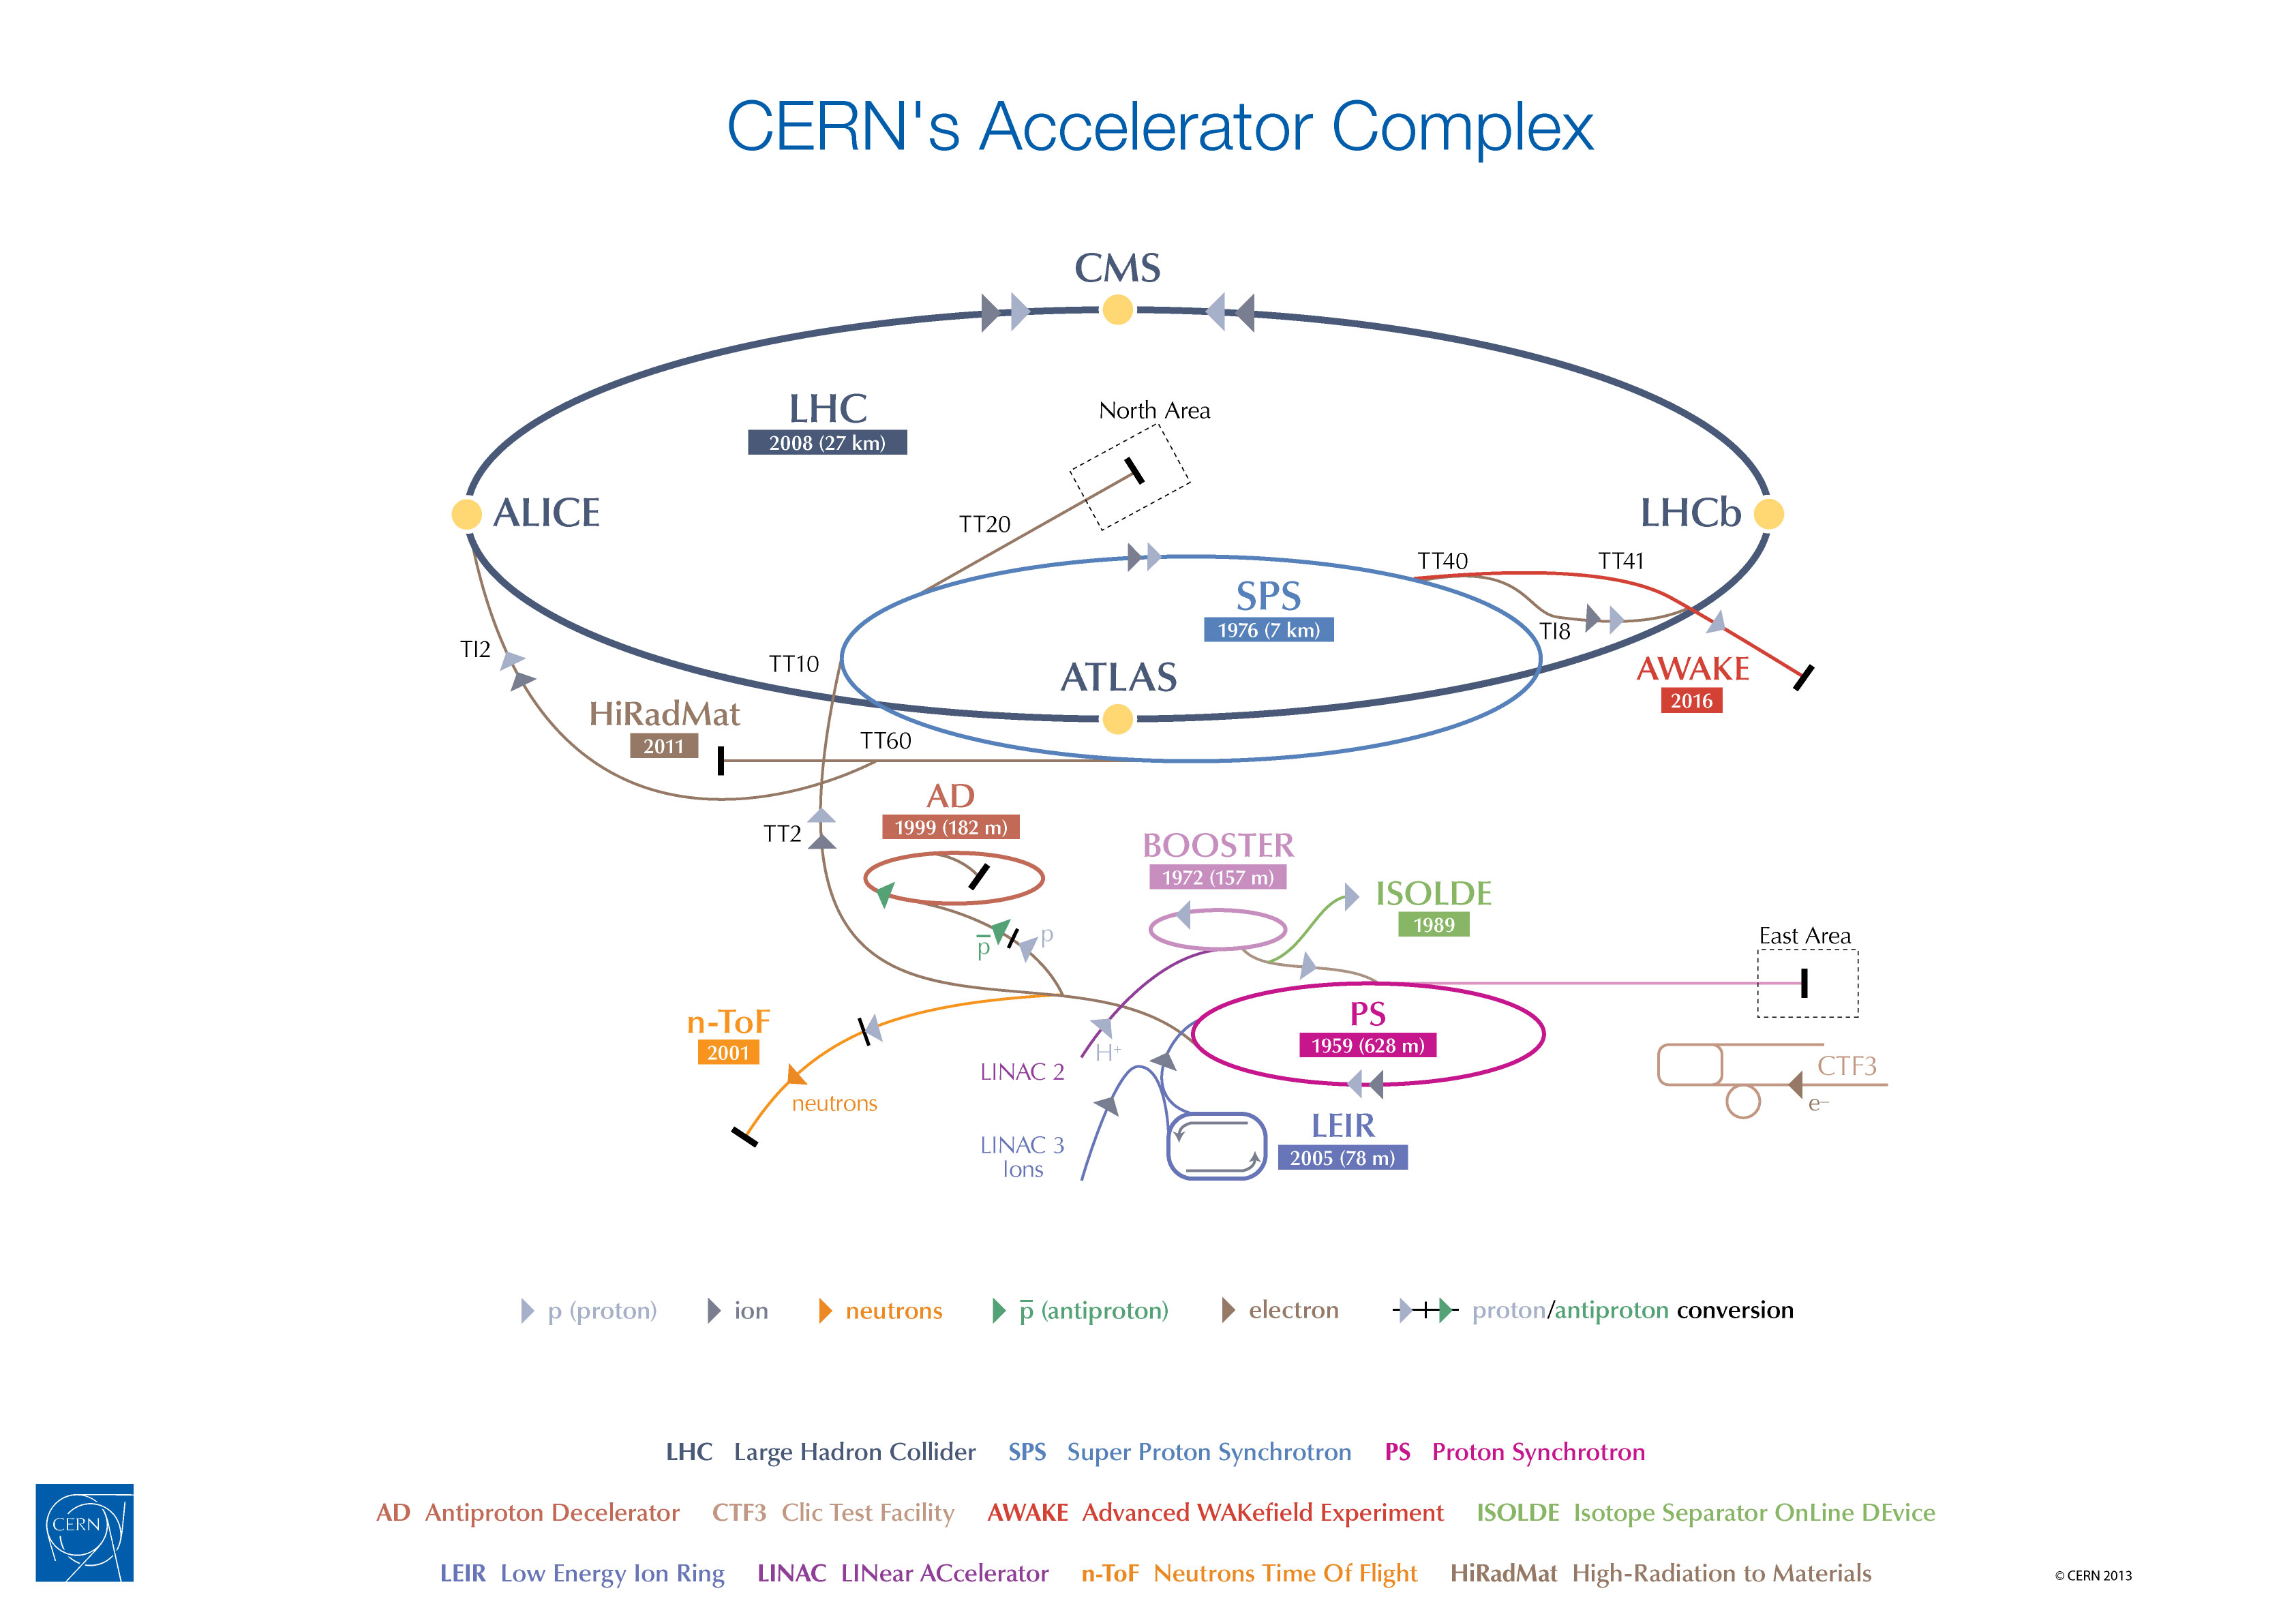
\includegraphics[scale = 0.75]{figs/Detector/LHC.jpg}
\caption{Layout of the LHC (Large Hadron COllider).}
\label{LHC}
\end{center}
\end{figure} 

The CMS and ATLAS are the two general purpose detectors to analyse the particles produced by collisions in the accelerator i.e. to cover the widest possible range of physics at the LHC,
from the search for the Higgs boson, supersymmetry (SUSY) to extra dimensions. How a prototype detector shapes into a real detector can be seen in comparison to a real detector at LHC, so we discuss below, CMS in this context.
\subsection{CMS}
The CMS (Compact Muon Solenoid) detector  is 21 m long, 15 m wide and 15 m high, shown in Figure \ref{CMS}. It is built around a huge solenoid magnet. A cylindrical coil of superconducting cable generates a magnetic field of 4 Tesla. The magnetic field is confined by a steel ``yoke'' that forms the bulk of the detector's weight of 12,500 tonnes. 

\begin{figure}[h!]
\begin{center} 
\includegraphics[scale = 0.85]{figs/Detector/CMS1.jpg}
\caption{Overview of the CMS (Compact Muon Solenoid) Detector .}
\label{CMS}
\end{center}
\end{figure}

 \begin{itemize}
\item
The particles produced from the collisions at LHC, first pass through a tracker which is made up of silicon entirely. It is a cylinder of 6m and a diameter of 2.6m. It tracks their positions and is helpful in measuring their momentum. There are calorimeters outside the tracker that measure the energy of particles. In measuring the momentum, the tracker should interfere with the particles as little as possible, whereas the calorimeters are specifically designed to stop the particles in their tracks.
 \item
The Electromagnetic Calorimeter (ECAL) is made of lead tungstate (PbWO$_{4}$) which is a very dense material that produces light when a particle hits on it. The energy of the produced photons and electrons is measured by using silicon avalanche photodiodes in the barrel and cacuum photo diodes in the endcaps. The electromagnetic calorimeter comprises of 61200 lead tungstate crystals mounted in the central barrel part and 7324 crystals in each of the two endcaps. Lead tungstate scintillating crystals were chosen because of their short radiation length \footnote{Radiation length describes the longitudinal shower development. It is a scaling variable for the probability of occurrence of bremsstrahlung, pair production and for the variance of the angle of multiple scattering. The characteristic amount of matter traversed for these related interactions is called the radiation length.} ($X_{0} = 0.89cm$) and
small Moli$\acute{e}$re (2.2 cm) radius \footnote{ A characteristic constant of a  material describing its transverse dimensions of the electromagnetic showers which are initiated by an incident high energy electron or photon.}, in order to stop all
electrons and photons within a minimal depth of the material.
This enabled the CMS collaboration to build a compact calorimeter within the solenoid.

\item
The Hadron Calorimeter (HCAL) is designed to detect any particle made up of quarks (the basic building blocks of protons and neutrons).Hadronic barrel (HB) and hadronic endcap (HE) calorimeters are sampling calorimeters with 50mm thick copper (selected because of its density) absorber plates which are interleaved with 4mm scintillator sheets. HB is made of two 4.4m length half-barrels, and HE has two large structures, situated at each end of the barrel detector and within the region of high magnetic field. Hadronic forward (HF) calorimeter are two in number and are situated at each extreme of the CMS
detector. It is made of steel absorbing plates and quartz fibers are inserted into
them. The passage of charged particles through the quartz fibers produces Cerenkov
light signals, which are used to measure the energy of the jets.

 \item
The Superconducting magnet is 13m long and 6m in diameter, and its refrigerated superconducting
niobium-titanium coils, cooled at -270$^{\circ}$C, produces a magnetic field of 4 Teslas. This intense solenoidal field is the main key to design the experiment as it is responsible for the compactness and cylindrical symmetry of the detector. The size of the magnet allows the tracker and calorimeters to be placed inside its coil, resulting in an overall compact detector. The magnetic field is obtained by a solenoid because  with the field parallel to
the beam  the bending of the muon tracks is in the transverse plane and thus making the measurement of momenta possible.

\item
As the name suggests CMS is also designed to detect muons. The outer part of the detector is the  magnet ``return yoke'', which confines and guides the magnetic field.  The four layers of detectors are interleaved with the iron  which also provides the detector's support structure. CMS was designed in fifteen separate sections or ``slices'' that were built on the surface and lowered down ready-made into the cavern. 
\end{itemize}

The basic structure of a prototype detector forms the basis for the conctruction of any real detector. There can be some changes in the design of the detector according to the needs of the aim of the experiment to be carried out with the detector.
The various detectors of the LHC have different aims which are given below in a brief way :
\begin{itemize}
\item  
The $\bf{ATLAS}$ (A Toroidal LHC Apparatus) detector shown in Figure \ref{ATLAS} is searching for new discoveries in the head-on collisions of protons with an extraordinarily high energy. The objective is to observe the phenomena that involve highly massive particles which were not observable using earlier lower-energy accelerators and the particles that could make up dark matter. It has six different detecting subsystems that identify particles and measure their momenta and energy.
 
\begin{figure}[h!]
\begin{center} 
\includegraphics[scale = 0.30]{figs/Detector/ATLASF.jpg}
\caption{Overview of the ATLAS (A Toroidal LHC Apparatus) Detector.}
\label{ATLAS}
\end{center}
\end{figure}
\item

The $\bf{ALICE}$ (A Large Ion Collider Experiment) detector shown in Figure \ref{ALICE}(a) is a heavy-ion detector which focuses on QCD. It aims to collide lead ions to recreate the conditions just after the Big Bang under laboratory conditions. It is designed to study a state of matter known as quark-gluon plasma, which is believed to have existed soon after the Big Bang. The ALICE collaboration plans to study the quark-gluon plasma as it expands and cools, observing how it progressively gives rise to the particles that constitute the matter of our Universe today.

\begin{figure}[h!]
\begin{center} 
\includegraphics[scale = 0.40]{figs/Detector/alice.jpg}%
\includegraphics[scale = 0.50]{figs/Detector/LHCb.jpg}

\caption{(a) Overview of the ALICE (A Large Ion Collider Experiment) Detector. (b)Overview of the LHCb (Large Hadron Collider beauty) Detector.}
\label{ALICE}
\end{center}
\end{figure}

\item
The $\bf{LHCb}$ (Large Hadron Collider beauty) experiment Figure \ref{ALICE}(b) will investigate the slight differences between matter and antimatter by studying a type of particle called the beauty or b quark. It will help us to understand why the Universe appears to be composed almost entirely of matter and not the antimatter. The LHCb experiment uses a series of sub-detectors to detect mainly forward particles istead of surrounding the entire collision point with an enclosed detector. An abundance of different types of quark will be created by the LHC before they decay quickly into other forms. To catch the b-quarks, LHCb has developed sophisticated movable tracking detectors close to the path of the beams circling in the LHC. It is also dedicated to precision measurements of CP violation.


\item
The $\bf{LHCf}$ (Large Hadron Collider forward) uses forward particles created inside the LHC as a source to simulate cosmic rays in laboratory conditions. Cosmic rays are naturally occurring charged particles from outer space that constantly bombard the Earth's atmosphere. They collide with nuclei in the upper atmosphere, leading to a cascade of particles that reaches ground level. LHCf will study the collisions inside the LHC which cause similar cascades of particles and it will to interpret large-scale cosmic-ray experiments.

\item
The  $\bf{TOTEM}$ (TOTal Elastic and diffractive cross section Measurement) studies forward particles to focus on physics that is not accessible to the general-purpose experiments. It will measure the total pp cross-section in a luminosity-independent method and study elastic and diffractive scattering at the LHC. TOTEM will also complement the results obtained by the CMS detector and by the other LHC experiments overall.

\end{itemize}
\end{comment}
